\documentclass[12pt,twoside, a4paper, twocolumn]{article}
\usepackage[utf8]{inputenc}
\usepackage[brazil]{babel}
\usepackage[margin = 0.5in]{geometry}
\usepackage{amsmath}
\usepackage{amsthm}
\usepackage{amssymb}
\usepackage{amsthm}
\usepackage{setspace}
\usepackage[americanvoltages,fulldiodes,siunitx]{circuitikz}
\usepackage{lipsum}
\usepackage{pgfplots}
\usepackage{ifthen}
\usepackage{adjustbox}
\usepackage[section]{placeins}
\usepackage{hyperref}
\usepackage{graphicx}
\usepackage{adjustbox}
\pgfplotsset{compat=newest}
\graphicspath{ {./images/} }
%  #1 color - optional #2 x_0 #3 y_0 #4 x_f #5 y_f #6 name - optional  #7 true if adding lines to axis
\newcommand{\drawvector} [9] [color=cyan] {
\draw[line width=1.5pt,#1,-stealth](axis cs: #2, #3)--(axis cs: #4, #5) node[anchor=south west]{$#6$};
\ifthenelse{\equal{#7}{true}}{
\draw[line width=1pt,#1, dashed](axis cs: #4, #5)--(axis cs: #4, 0) node[anchor= north west]{$#8$};
\draw[line width=1pt,#1, dashed](axis cs: #4, #5)--(axis cs: 0, #5) node[anchor=south east]{$#9$};
}
{}
}
\newcommand\deriv[2]{\frac{\mathrm d #1}{\mathrm d #2}}
\title{Decimo  Relatório de Física Experimental 2}
\author{Henrique da Silva \\ hpsilva@proton.me}
\date{\today}
\pgfplotsset{width = 10cm, compat = 1.9}
\begin{document}
\maketitle
\pagenumbering{gobble}
\newpage
%pagenumbering{roman}
\tableofcontents
\newpage

\section{Introdução}

\paragraph*{Neste relatório, vamos discutir difracao de fendas simples, redes de difracao, e decomposicao espectral.}

\paragraph*{Também discutiremos alguns circuitos retificadores com diodos.}

\paragraph*{Todos arquivos utilizados para criar este relatório, é o relatório em si estão em:  \url{https://github.com/Shapis/ufpe_ee/tree/main/4th semester/}}


\section{Difracao de Fraunhofer}


\subsection{Tabela de dados inicial}

\begin{center}
  \begin{tabular}{ |c|c|c| }
    \hline
    $Paquimetro$          & $Primeiro\,Minimo$    \\
    $(0.10 \pm 0.05)\,mm$ & $(1.55 \pm 0.05)\,cm$ \\
    $(0.20 \pm 0.05)\,mm$ & $(1.15 \pm 0.05)\,cm$ \\
    $(0.30 \pm 0.05)\,mm$ & $(0.50 \pm 0.05)\,cm$ \\
    $(0.40 \pm 0.05)\,mm$ & $(0.40 \pm 0.05)\,cm$ \\
    $(0.50 \pm 0.05)\,mm$ & $(0.35 \pm 0.05)\,cm$ \\
    \hline
  \end{tabular}
\end{center}


\subsection{Analise Teorica}
\paragraph*{Para prosseguirmos precisamos lembrar das seguintes relacoes:}

\begin{equation}
  \begin{aligned}
     & a * \sin \theta = m \lambda     \\
     & m = 1                           \\
     & a * \sin \theta = \lambda       \\
     & \sin \theta = \frac{\lambda}{a} \\
  \end{aligned}
\end{equation}

\paragraph*{Que nos da uma relacao linear se consideramos ao inves de $a$, consideramos seu inverso $\gamma = 1/a$.}

\begin{equation}
  \sin \theta = \lambda \gamma
\end{equation}


\subsection{Tabela de dados extendida}
\begin{center}
  \begin{tabular}{ |c|c|c|c|c| }
    \hline
    $a$                   & $1/a$                 & $y$                   & $x$             & $\sin{\theta}$ \\
    $(0.10 \pm 0.05)\,mm$ & $(10.0 \pm 2)mm^{-1}$ & $(1.55 \pm 0.05)\,cm$ & $(217 \pm 5)cm$ & $(0.0071 \pm)$ \\
    $(0.20 \pm 0.05)\,mm$ & $(5.0 \pm 2)mm^{-1}$  & $(1.15 \pm 0.05)\,cm$ & $(217 \pm 5)cm$ & $(0.0053 \pm)$ \\
    $(0.30 \pm 0.05)\,mm$ & $(3.3 \pm 2)mm^{-1}$  & $(0.50 \pm 0.05)\,cm$ & $(217 \pm 5)cm$ & $(0.0023 \pm)$ \\
    $(0.40 \pm 0.05)\,mm$ & $(2.5 \pm 2)mm^{-1}$  & $(0.40 \pm 0.05)\,cm$ & $(217 \pm 5)cm$ & $(0.0018 \pm)$ \\
    $(0.50 \pm 0.05)\,mm$ & $(2.0 \pm 2)mm^{-1}$  & $(0.35 \pm 0.05)\,cm$ & $(217 \pm 5)cm$ & $(0.0016 \pm)$ \\
    \hline
  \end{tabular}
\end{center}

\subsection{Grafico de $\sin{\theta}$ vs $1/a$}

\begin{adjustbox}{scale=0.70}
  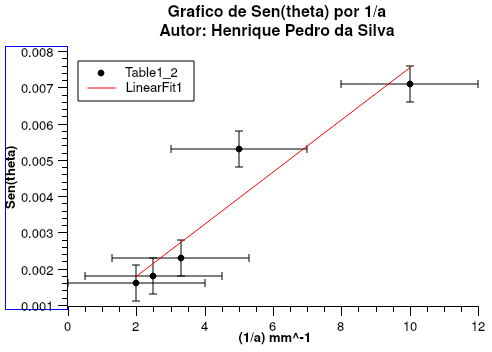
\includegraphics{Graph1.png}
\end{adjustbox}

\paragraph*{Podemos ver de fato, que como esperado obtemos uma relacao linear entre $\sin{\theta}$ e $1/a$.}

\paragraph*{E o coeficiente angular da reta, encontrado foi de $717.4$. Porem, com error na ordem de $100$.}

\paragraph*{Logo podemos afirmar que o comprimento de onda encontrado foi de $700 \pm 100$ nm. Que esta dentro do esperado.}

\paragraph*{E seu percentual de desvio foi de $10\%$ aproximadamente.}

\newpage






\end{document}